\documentclass{article}
\usepackage{graphicx}
\usepackage{amsfonts,amsmath,amssymb}

\begin{document}
 

\section{A comparison to real data}

%intention
We now seek to explore a real dataset to make a first order comparison with the assumptions and predictions of our model. Currently EHT datasets are not public, so we have opted to use a 3.5~mm VLBA dataset from the public, online VLBA archive. We chose an observation of SgrA* and nearby calibrator NRAO530. 

\subsection{Phases and coherence}

%Coherence times 
In our canonical simulations (section~\ref{can:sim}) we assumed a constant zenith coherence time of $t_0 = 10$~s throughout the duration of the observation.  Scaling up to 3.5~mm for the VLBA, this translates to $t_0 \approx 25$~s, with the caveat that, on average, EHT stations are situated in locations with more stable atmospheres than VLBA stations. Fig.~\ref{fig:coherence} shows a normalised histogram of coherence times towards NRAO530 for all baselines and scans. We find a mean and standard deviation of the coherence times to be $(\mu, \sigma)_{\rm t_0} = (8.87,6.09)$. However this is coherence for baselines not stations... The coherence times seem to be fairly consistent throughout the observation.

\begin{figure}[h]
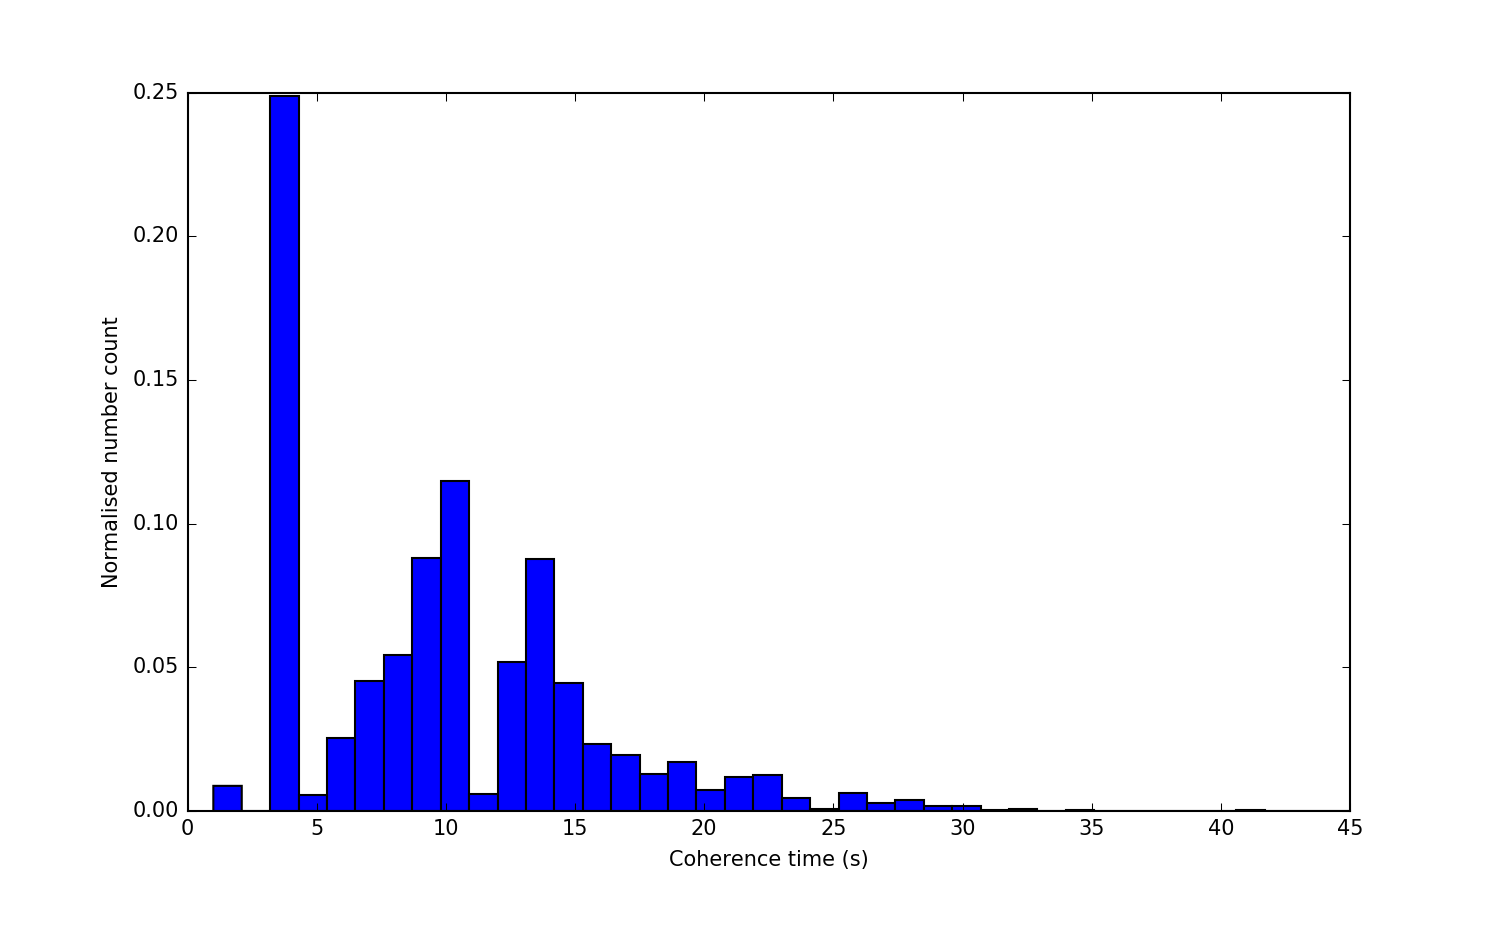
\includegraphics[width=\columnwidth]{Images/Coherence_time_NRAO530ff}
\caption{Normalised histogram of the coherence times for 87~GHz VLBA observation of NRAO530. The coherence times were generated using the {\sc aips} {\sc coher} task. The mean and standard deviation of the coherence times, $(\mu, \sigma) = (8.87,6.09)$. \label{fig:coherence}%
}
\end{figure}


An inspection of the observation weather tables shows a ground windspeed  $(\mu, \sigma)_v = (2.5, 1.8)$~m/s. This speed is too low to account for the above coherence time and hence indicates that most of the turbulence originates higher up in the troposphere.


%Inspectation of the histograms of phase differences
Trying to compare the scatter on the visibility phase difference between consecutive times and to the theoretical value (now that we know the mean coherence time and assuming the canonical turbulent exponent). With an estimate of the coherence and assuming the canonical value for the turbulent exponent $\beta = 5/6$, we estimate, for $t_int \approx 1$, ${\sigma_\phi \approx (t_{\int}/t_0)^{5/6} \approx 9}^\circ$. Data perspective is more complicated..Without an additional delay search, $\sigma_\phi$ (data) will be much higher... can one apply the delay found by AIPS COHER to the UVFITS file? ...[frequency averaging procedure?] averaging over channel but taking the difference in time. 

\subsection{Closure phase} 

How large is the uncertainty on the closure phase. Is this consistent with just a thermal noise prediction? If it is not consistent it's difficult to isolate what would dominate this. With only 1 epoch of observation we won't be able to see any ISM variations.


\subsection{Amplitude}

What is the variability in the visibility amplitude? How significant is the stochastic variation? How does it compare to thermal noise?

Are there any obvious systematics in the data? 


\end{document}
